% vim: set tw=0:
\documentclass{beamer}
\usepackage{graphicx}

% Reasonable themes:
% Antibes Bergen Berkeley Berlin Frankfurt Goettingen Ilmenau Luebeck Malmoe
% Montpellier PaloAlto Rochester Singapore Szeged Warsaw bars boxes
% compatibility default lined plain shadow sidebar split tree
% And these ones include the author's name on every slide:
% Berkeley

% Declare themes.
\mode<presentation>
\usetheme{UWHEP}

% Personal macros.
\newcommand{\email}[1]{{\texttt #1}}
\newcommand{\newframe}[1]{\section{#1}
    \frametitle{\sc{#1}}}
\newcommand{\subframe}[1]{\subsection{#1}
    \frametitle{\sc{#1}}}
\newcommand{\supers}[1]{\ensuremath{^\textrm{#1}}}
\newcommand{\subs}[1]{\ensuremath{_\textrm{#1}}}
\newcommand{\ca}{\ensuremath{\sim}}

% Author information.
\title{T2 Status}
\author[Maier, Mohapatra]{
    Will Maier \and Ajit Mohapatra\\ 
    {\tt wcmaier@hep.wisc.edu}\\
    {\tt ajit@hep.wisc.edu}}
\institute[Wisconsin]{University of Wisconsin - High Energy Physics}
\date{2008.10.28}
\logo{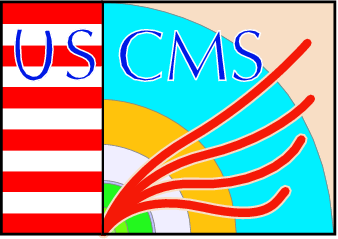
\includegraphics[height=0.6cm]{../../../Graphics/USCMS_logo.png}\hspace{.1cm}
\includegraphics[height=0.75cm]{../../../Graphics/UW_logo.png}}

\begin{document}

\begin{frame}
    \titlepage
\end{frame}

%\section{Overview}
%\begin{frame}
%    \tableofcontents
%\end{frame}

\section{Facilities}
\subsection{Software and Storage}
\begin{frame}
\frametitle{}
\begin{itemize}
    \item Deployed new storage nodes (10 x 24 TB)
    \begin{itemize}
        \item Nodes racked; half installed
        \item Running burn-in
    \end{itemize}
    \item Began preparations for dCache 1.9
    \begin{itemize}
        \item Reconciled upstream changes with local modifications
        \item Upgrade planned for early January (unless bugs in 1.8 prompt earlier action)
    \end{itemize}
    \item Tightened RSV configuration
    \item Set up GSISSH
    \begin{itemize}
        \item Plan to retire local {\tt grid-xterm}
        \item Requires valid shells in {\tt /etc/passwd}
    \end{itemize}
    \item Enabled {\tt osg\_sbgrid}
\end{itemize}
\end{frame}

\subsection{Production and Monitoring}
\begin{frame}
\frametitle{}
\begin{itemize}
     \item JobRobot: OK
     \item SAM: OK
     \item RSV: OK
     \item PhEDEx:
     \begin{itemize}
        \item \ldots{}
     \end{itemize}
     \item MC Production: \ldots{}
\end{itemize}
\end{frame}

\end{document}
